% --------------------------------------------------------------------------------
% ---------------------------------  Preamble  -----------------------------------
% --------------------------------------------------------------------------------

\documentclass{article}

\usepackage{microtype}

\usepackage[letterpaper, margin=0.75in]{geometry}
\usepackage{graphicx}               % to insert figures
\usepackage[table,x11names]{xcolor} % colors for e-copies
\usepackage{subcaption}             % subfigures
\usepackage{placeins}               % Float barriers
\usepackage{booktabs}
\usepackage{array}
\usepackage{caption}
\usepackage{rotating}
\usepackage{multicol}
\usepackage{multirow}
\usepackage{titlesec}
\usepackage{hyperref}               % PDF hyperreferences
\usepackage{titling}
\usepackage{tikz}
\usetikzlibrary{shapes.geometric}
\usetikzlibrary{calc}
\usepackage[T1]{fontenc}
\usepackage{ifthen}

\newcommand{\mysectiontitle}{}
\newcommand{\newsection}[2]{\renewcommand{\mysectiontitle}{#2}\section{#1}}

\titleformat{\paragraph}
{\normalfont\normalsize\bfseries}{\theparagraph}{1em}{}
\titlespacing*{\paragraph}
{0pt}{3.25ex plus 1ex minus .2ex}{1.5ex plus .2ex}

\newcommand{\Vline}[1]{}
\newcommand{\Hline}[1]{\hline}

\title{Skirmishers}
\author{}
\date{}

\newcommand{\outworldsMode}{mode-web}

% --------------------------------------------------------------------------------
% ---------------------------------  Document  -----------------------------------
% --------------------------------------------------------------------------------

\begin{document}

\makeatletter
\Tag{TITLE+}{\@title}

\begin{center}
  \fontsize{30}{37}\bfseries\selectfont\MakeUppercase{War Department}
  \fontsize{50}{60}\bfseries\selectfont\MakeUppercase{Skirmishers}
  \fontsize{30}{37}\bfseries\selectfont\MakeUppercase{GM 1-1}

  \LARGE\bfseries{Game Manual}
\end{center}

% --------------------------------------------------------------------------------
\newsection{Introduction}{introduction}
% --------------------------------------------------------------------------------

Infantry troopers can wear power armor in \emph{Skirmishers}.
This section relies upon rules from the Advanced Infantry section.


% --------------------------------------------------------------------------------
\subsubsection*{Unit Card}
% --------------------------------------------------------------------------------

The unit card shows the current capabilities of a trooper in power armor and tracks damage.
A unit card can be formatted in any way so long as it contains all the essential information.
Below is a sample unit card for a power armor trooper.

\begin{figure}[H]
  \centering
  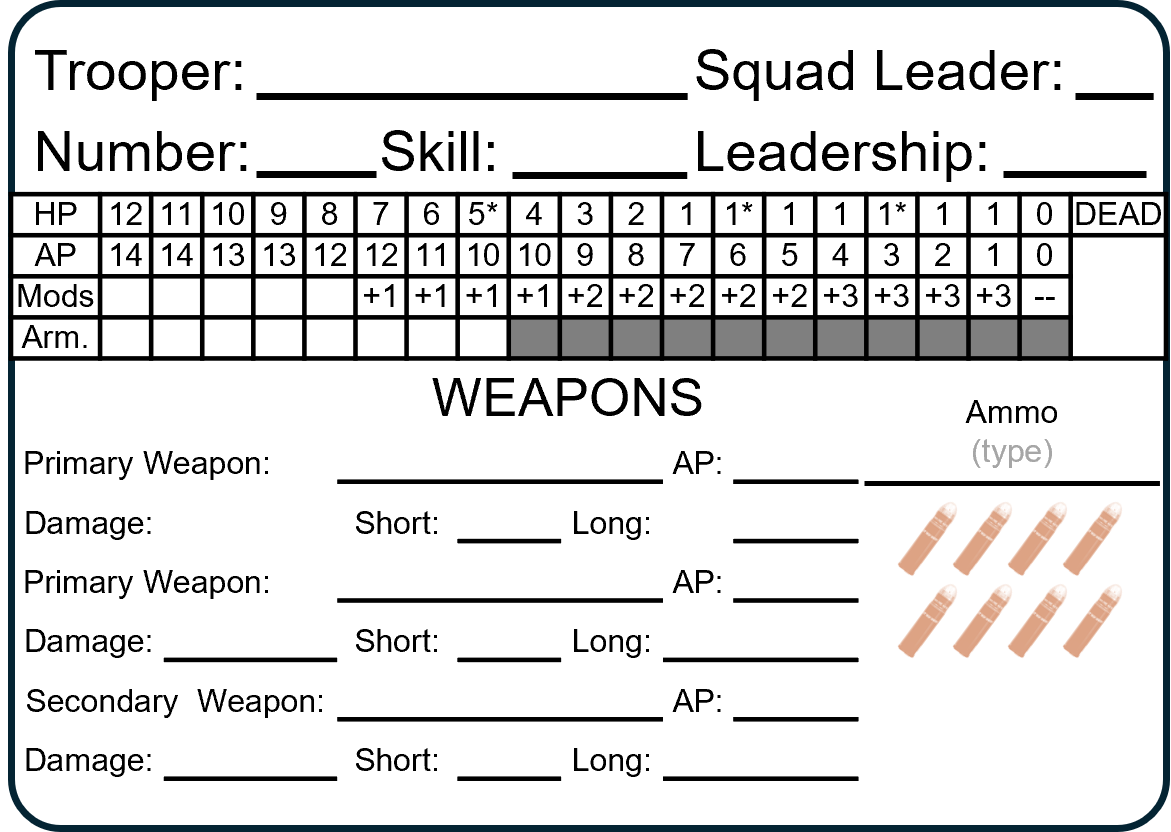
\includegraphics[alt='Sample Power Armor Trooper', width=5.63in, height=4in]{img/PowerArmorTrooper.png}
  \caption*{Power Armor Trooper Unit Card}
\end{figure}

There are a few key differences between the standard trooper unit card and a power armor trooper unit card.

Standard power armor has 6 cells of armor.
Basic power armor has only 4 cells of armor and heavy power armor has 8 cells of armor.
All other cells of armor should be marked off before the game.

Power armor troopers ignore bludgeoning damage (\textbackslash).
However, 9 or more points of bludgeoning damage in a single turn will knock a power armor trooper prone.
Standard damage (X) destroys armor before damaging HP cells.
If a single attack does more damage than the remaining armor, first mark all remaining armor and then mark HP cells starting with the 12 HP cell.

Once all of the armor has been destroyed, then the trooper's HP cells are marked.
Power armor protects the trooper, giving them more HP than a basic trooper.
HP cells are fully crossed out when the trooper takes standard damage (X).
The current HP of the trooper is given by the first cell to the right of the highest fully marked HP cell.
For example, if the trooper has HP 10, 9, and 6 marked off, their current HP is 5.
When marking damage, you still roll 2D6 and apply damage starting with the first unmarked HP cell to the right of the rolled value.

The HP cells marked with * indicate significant damage to the power armor.
When one of these cells is fully marked, the opponent may choose one of the weapon systems to disable on the power armor suit.
When two of these cells have been fully marked, the jet pack on the suit no longer functions.

Total action points (AP) for the trooper are given in the AP section.
Power armor greatly extends the capabilities of troopers, giving them more AP.
Use the value in the column corresponding to the trooper's current HP.
For example, if the trooper has 5 HP, then they have only 10 AP.

As with standard troopers, green troopers in power armor reduce all of their AP values by 1, while veteran troopers increase all values by 1 and elite troopers increase all values by 2.

Similarly, the modifier section tracks the current modifier for the trooper's target numbers based upon current HP.
For example, if the trooper has 5 HP, then add +1 to all target numbers.

Basic and standard power armor comes equipped with a jet pack.
Heavy power armor is too bulky to use a jet pack.

The weapons and equipment section list the primary and secondary weapons the trooper is equipped with, along with their damage values and range brackets.
Power armor troopers cannot use grenades but may use satchel changes.

The leadership section lists the squad leader for the trooper and their leadership score.
This section contains the information required for morale checks.


% --------------------------------------------------------------------------------
\subsubsection*{Weapons and Equipment}
% --------------------------------------------------------------------------------

Troopers carry one primary weapon, one secondary weapon, and 4 hand grenades.
All troopers have a helmet and combat knife.
The combat knife is assumed to be attached as a bayonet if the trooper is carrying a rifle or SMG.
Troopers may carry additional equipment in some cases.

\paragraph*{Primary Weapons}

Each trooper carries a single primary weapon.
Troopers can use the following primary weapons:

\begin{table}[H]
\ifthenelse{\not \equal{\outworldsMode}{mode-web}}{\fontfamily{Montserrat-LF}}{\small}\selectfont
\centering
\newcolumntype{R}[1]{>{\raggedleft\let\newline\\\arraybackslash\hspace{0pt}}m{#1}}
\begin{tabular}{!{\Vline{1pt}} m{6em} !{\Vline{1pt}} R{4.5em} !{\Vline{1pt}} R{6.5em} !{\Vline{1pt}} R{6.5em} !{\Vline{1pt}}}
\Hline{1pt}
\rowcolor{black!30}  \bfseries{Weapon} & \bfseries{Damage} & \bfseries{Short Range} & \bfseries{Long Range} \\
\Hline{1pt}
SMG*          & 3X &  5 &  17  \\
Rifle         & 4X & 26 &  85  \\
Laser SMG*    & 4X & 43 & 127  \\
Laser Rifle   & 5X & 66 & 232  \\
Long Rifle    & 6X & 30 & 102  \\
Gyrojet Rifle & 6X & 31 & 137  \\
\Hline{1pt}
\end{tabular}
\caption*{Primary Weapons}
\end{table}

Note, the SMG and Laser SMG are burst fire weapons and can fire into the same firing arc multiple times.
All other weapons may only fire into a firing arc once per turn.

\paragraph*{Secondary Weapons}

Each trooper may carry a single secondary weapon.
Troopers can use the following ranged secondary weapons:

\begin{table}[H]
\ifthenelse{\not \equal{\outworldsMode}{mode-web}}{\fontfamily{Montserrat-LF}}{\small}\selectfont
\centering
\newcolumntype{R}[1]{>{\raggedleft\let\newline\\\arraybackslash\hspace{0pt}}m{#1}}
\begin{tabular}{!{\Vline{1pt}} m{6em} !{\Vline{1pt}} R{4.5em} !{\Vline{1pt}} R{6.5em} !{\Vline{1pt}} R{6.5em} !{\Vline{1pt}}}
\Hline{1pt}
\rowcolor{black!30}  \bfseries{Weapon} & \bfseries{Damage} & \bfseries{Short Range} & \bfseries{Long Range} \\
\Hline{1pt}
Pistol        & 2X &  7 & 20  \\
Auto Pistol*  & 3X &  6 & 22  \\
Laser Pistol  & 4X & 11 & 40  \\
\Hline{1pt}
\end{tabular}
\caption*{Ranged Secondary Weapons}
\end{table}

Note, the auto pistol is a burst fire weapon and can fire into the same firing arc multiple times.
All other weapons may only fire into a firing arc once per turn.

Troopers can use the following melee secondary weapons:

\begin{table}[H]
\ifthenelse{\not \equal{\outworldsMode}{mode-web}}{\fontfamily{Montserrat-LF}}{\small}\selectfont
\centering
\newcolumntype{R}[1]{>{\raggedleft\let\newline\\\arraybackslash\hspace{0pt}}m{#1}}
\begin{tabular}{!{\Vline{1pt}} m{7.2em} !{\Vline{1pt}} R{5em} !{\Vline{1pt}} R{6.5em} !{\Vline{1pt}} R{6.5em} !{\Vline{1pt}}}
\Hline{1pt}
\rowcolor{black!30}  \bfseries{Weapon} & \bfseries{Damage} & \bfseries{Short Range} & \bfseries{Long Range} \\
\Hline{1pt}
Fists         & (AP/2)\textbackslash & 1 & --  \\
Bayonet/Knife & 3X                   & 1 & --  \\
Blackjack     & 5\textbackslash      & 1 & --  \\
Club          & 1X, 4\textbackslash  & 1 & --  \\
Stun Baton    & 8\textbackslash      & 1 & --  \\
Sword         & 4X                   & 1 & --  \\
Vibroblade    & 5X                   & 1 & --  \\
\Hline{1pt}
\end{tabular}
\caption*{Melee Secondary Weapons}
\end{table}

A trooper always has their fists and a bayonet/knife.
The other melee weapons take the place of a secondary weapon.

\paragraph*{Explosive Weapons}

Troopers can use the following explosives:

\begin{table}[H]
\ifthenelse{\not \equal{\outworldsMode}{mode-web}}{\fontfamily{Montserrat-LF}}{\small}\selectfont
\centering
\newcolumntype{R}[1]{>{\raggedleft\let\newline\\\arraybackslash\hspace{0pt}}m{#1}}
\begin{tabular}{!{\Vline{1pt}} m{8em} !{\Vline{1pt}} R{4.9em} !{\Vline{1pt}} R{4.1em} !{\Vline{1pt}} R{4em} !{\Vline{1pt}} R{6.5em} !{\Vline{1pt}} R{6.5em} !{\Vline{1pt}}}
\Hline{1pt}
\rowcolor{black!30}  \bfseries{Weapon} & \bfseries{Damage} & \bfseries{AP Cost} & \bfseries{Ammo} & \bfseries{Short Range} & \bfseries{Long Range} \\
\Hline{1pt}
Hand Grenade   &    6X/3X/1X & AP      & 4 & AP   & --  \\
Satchel Charge &   10X/5X/2X & 3 or AP & 1 & AP/2 & --  \\
\Hline{1pt}
\end{tabular}
\caption*{Explosive Weapons}
\end{table}

The ammo column indicates how many rounds of ammunition come with the weapon.
The damage is given is descending order for the point of detonation, the adjacent dots, the dots 2 away from the detonation, and so on.
It takes 1 AP per dot to throw a hand grenade and it takes 2 AP per dot to throw a satchel charge.

A trooper carries 4 grenades in addition to their primary and secondary weapons.
A satchel charge is a secondary weapon, so a trooper cannot carry a ranged or melee secondary weapon if they are carrying a satchel charge.

\paragraph*{Body Armor}

Troopers can wear body armor.
A trooper ignores bludgeoning damage while wearing body armor and any cells of armor are destroyed before applying lethal damage to the trooper.

\begin{table}[H]
\ifthenelse{\not \equal{\outworldsMode}{mode-web}}{\fontfamily{Montserrat-LF}}{\small}\selectfont
\centering
\newcolumntype{R}[1]{>{\raggedleft\let\newline\\\arraybackslash\hspace{0pt}}m{#1}}
\begin{tabular}{!{\Vline{1pt}} m{6.5em} !{\Vline{1pt}} R{5em} !{\Vline{1pt}} R{4.5em} !{\Vline{1pt}}}
\Hline{1pt}
\rowcolor{black!30}  \bfseries{Armor Type} & \bfseries{Coverage} & \bfseries{AP Cost} \\
\Hline{1pt}
Basic    & 2 & 1  \\
Standard & 4 & 2  \\
Heavy    & 6 & 3  \\
\Hline{1pt}
\end{tabular}
\caption*{Body Armor AP Costs}
\end{table}

To equip body armor on a trooper, indicate the number of cells of body armor on the unit card and mark off all other cells of armor before the game.
Reduce the trooper's AP to account for the body armor.
For example, with standard body armor, leave 4 cells of armor on the unit card and reduce all values in the AP row by 2.


% --------------------------------------------------------------------------------
\subsubsection*{Movement}
% --------------------------------------------------------------------------------

Troopers may move and take special actions prior to taking any combat actions.

\paragraph*{Basic Movement}

Troopers can use a maximum of 8 AP for movement.
Troopers move between adjacent dots on the map so long as the the new location is on valid terrain and the path between the dots does not pass though an impassible obstacle, such as a solid high wall or the truck of a tree.

Movement between adjacent dots with no obstructions between them costs 1 AP.
Movement between adjacent dots with an obstruction between costs 2 AP.
Obstructions include objects that are shorter than a person, such as furniture, light vegetation, and low walls.

Troopers may only enter and exit buildings through doorways and windows.
Movement between adjacent dots that passes through a doorway costs 2 AP.
Movement between adjacent dots that passes through a window costs 4 AP; however troopers cannot voluntarily fall out of an upper story window or off of a building.

Troopers may use stairs and ladders to change levels in or on a building.
Movement between levels costs 3 AP.
The trooper stays on the same dot when changing levels.
The current level of the trooper should be tracked on the unit card or next to the miniature.

Troopers may hide behind solid obstructions, such as furniture and low walls.
It costs 1 AP to go prone.
It costs 2 AP to stand from a prone position.
Movement while prone costs double the standard AP.

\begin{table}[H]
\ifthenelse{\not \equal{\outworldsMode}{mode-web}}{\fontfamily{Montserrat-LF}}{\small}\selectfont
\centering
\newcolumntype{R}[1]{>{\raggedleft\let\newline\\\arraybackslash\hspace{0pt}}m{#1}}
\begin{tabular}{!{\Vline{1pt}} m{9em} !{\Vline{1pt}} R{4.5em} !{\Vline{1pt}}}
\Hline{1pt}
\rowcolor{black!30}  \bfseries{Movement Type} & \bfseries{AP Cost} \\
\Hline{1pt}
Standard         & 1   \\
Obstructed       & 2   \\
Through door     & 2   \\
Through window   & 4   \\
Change level     & 3   \\
Go prone         & 1   \\
Stand from prone & 2   \\
Move while prone & 2x  \\
\Hline{1pt}
\end{tabular}
\caption*{Movement AP Costs}
\end{table}

\paragraph*{Special Actions}

A trooper may take the following special actions during their movement:

\begin{table}[H]
\ifthenelse{\not \equal{\outworldsMode}{mode-web}}{\fontfamily{Montserrat-LF}}{\small}\selectfont
\centering
\newcolumntype{R}[1]{>{\raggedleft\let\newline\\\arraybackslash\hspace{0pt}}m{#1}}
\begin{tabular}{!{\Vline{1pt}} m{11em} !{\Vline{1pt}} R{4.5em} !{\Vline{1pt}}}
\Hline{1pt}
\rowcolor{black!30}  \bfseries{Action} & \bfseries{AP Cost} \\
\Hline{1pt}
Change Weapon      & 3  \\
Exchange Equipment & 6  \\
\Hline{1pt}
\end{tabular}
\caption*{Special Action AP Costs}
\end{table}

A trooper can only have one weapon active at a time.
It costs 3 AP to change active weapons, including to change to an explosive.
A trooper automatically switches back to their primary or secondary weapon after using a grenade or satchel charge, for 0 AP.

Troopers may exchange weapons or equipment.
It costs 6 AP to take a weapon or equipment from another trooper, including a dead or unconscious trooper.
A trooper cannot exceed the basic carrying capabilities given on their unit card.
A trooper may drop weapons or equipment for 0 AP; however, any trooper, friendly or enemy, may pick up the dropped weapon or equipment.


% --------------------------------------------------------------------------------
\subsubsection*{Combat}
% --------------------------------------------------------------------------------

Power armor troopers largely use the same rules as standard troopers.

\paragraph*{Firing Arcs}

Power armor troopers may place firing arcs for all of their weapons.
If a weapon does not have a firing arc, then that weapon cannot fire.
If one of a power armor trooper's weapons is an explosive, this trooper may use the explosive and establish firing arcs with their other weapons.

\paragraph*{Hand to Hand Combat}

It costs 5 AP to make a hand to hand attack.
Power armor trooper fists are more effective at dealing damage.

\begin{table}[H]
\ifthenelse{\not \equal{\outworldsMode}{mode-web}}{\fontfamily{Montserrat-LF}}{\small}\selectfont
\centering
\newcolumntype{R}[1]{>{\raggedleft\let\newline\\\arraybackslash\hspace{0pt}}m{#1}}
\begin{tabular}{!{\Vline{1pt}} m{6em} !{\Vline{1pt}} R{5em} !{\Vline{1pt}} R{6.5em} !{\Vline{1pt}} R{6.5em} !{\Vline{1pt}}}
\Hline{1pt}
\rowcolor{black!30}  \bfseries{Weapon} & \bfseries{Damage} & \bfseries{Short Range} & \bfseries{Long Range} \\
\Hline{1pt}
Fists         & 1X, (AP/2)\textbackslash & 1 & - \\
\Hline{1pt}
\end{tabular}
\caption*{Power Armor Hand to Hand}
\end{table}

\paragraph*{Explosives}

Power armor troopers may use explosive weapons, but may not use hand grenades or smoke grenades.
Power armor troopers may pick up and use satchel charges.



\newpage

% --------------------------------------------------------------------------------
\newsection{System}{system}
% --------------------------------------------------------------------------------

Infantry troopers can wear power armor in \emph{Skirmishers}.
This section relies upon rules from the Advanced Infantry section.


% --------------------------------------------------------------------------------
\subsubsection*{Unit Card}
% --------------------------------------------------------------------------------

The unit card shows the current capabilities of a trooper in power armor and tracks damage.
A unit card can be formatted in any way so long as it contains all the essential information.
Below is a sample unit card for a power armor trooper.

\begin{figure}[H]
  \centering
  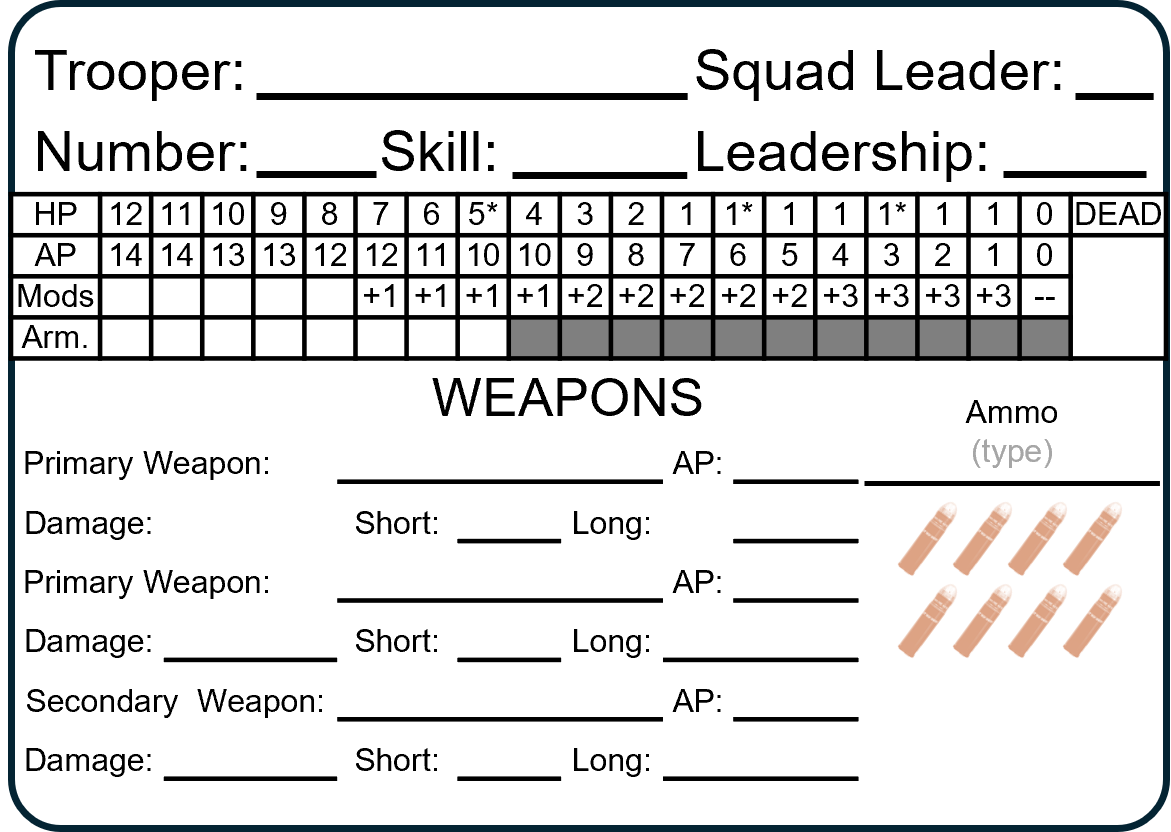
\includegraphics[alt='Sample Power Armor Trooper', width=5.63in, height=4in]{img/PowerArmorTrooper.png}
  \caption*{Power Armor Trooper Unit Card}
\end{figure}

There are a few key differences between the standard trooper unit card and a power armor trooper unit card.

Standard power armor has 6 cells of armor.
Basic power armor has only 4 cells of armor and heavy power armor has 8 cells of armor.
All other cells of armor should be marked off before the game.

Power armor troopers ignore bludgeoning damage (\textbackslash).
However, 9 or more points of bludgeoning damage in a single turn will knock a power armor trooper prone.
Standard damage (X) destroys armor before damaging HP cells.
If a single attack does more damage than the remaining armor, first mark all remaining armor and then mark HP cells starting with the 12 HP cell.

Once all of the armor has been destroyed, then the trooper's HP cells are marked.
Power armor protects the trooper, giving them more HP than a basic trooper.
HP cells are fully crossed out when the trooper takes standard damage (X).
The current HP of the trooper is given by the first cell to the right of the highest fully marked HP cell.
For example, if the trooper has HP 10, 9, and 6 marked off, their current HP is 5.
When marking damage, you still roll 2D6 and apply damage starting with the first unmarked HP cell to the right of the rolled value.

The HP cells marked with * indicate significant damage to the power armor.
When one of these cells is fully marked, the opponent may choose one of the weapon systems to disable on the power armor suit.
When two of these cells have been fully marked, the jet pack on the suit no longer functions.

Total action points (AP) for the trooper are given in the AP section.
Power armor greatly extends the capabilities of troopers, giving them more AP.
Use the value in the column corresponding to the trooper's current HP.
For example, if the trooper has 5 HP, then they have only 10 AP.

As with standard troopers, green troopers in power armor reduce all of their AP values by 1, while veteran troopers increase all values by 1 and elite troopers increase all values by 2.

Similarly, the modifier section tracks the current modifier for the trooper's target numbers based upon current HP.
For example, if the trooper has 5 HP, then add +1 to all target numbers.

Basic and standard power armor comes equipped with a jet pack.
Heavy power armor is too bulky to use a jet pack.

The weapons and equipment section list the primary and secondary weapons the trooper is equipped with, along with their damage values and range brackets.
Power armor troopers cannot use grenades but may use satchel changes.

The leadership section lists the squad leader for the trooper and their leadership score.
This section contains the information required for morale checks.


% --------------------------------------------------------------------------------
\subsubsection*{Weapons and Equipment}
% --------------------------------------------------------------------------------

Troopers carry one primary weapon, one secondary weapon, and 4 hand grenades.
All troopers have a helmet and combat knife.
The combat knife is assumed to be attached as a bayonet if the trooper is carrying a rifle or SMG.
Troopers may carry additional equipment in some cases.

\paragraph*{Primary Weapons}

Each trooper carries a single primary weapon.
Troopers can use the following primary weapons:

\begin{table}[H]
\ifthenelse{\not \equal{\outworldsMode}{mode-web}}{\fontfamily{Montserrat-LF}}{\small}\selectfont
\centering
\newcolumntype{R}[1]{>{\raggedleft\let\newline\\\arraybackslash\hspace{0pt}}m{#1}}
\begin{tabular}{!{\Vline{1pt}} m{6em} !{\Vline{1pt}} R{4.5em} !{\Vline{1pt}} R{6.5em} !{\Vline{1pt}} R{6.5em} !{\Vline{1pt}}}
\Hline{1pt}
\rowcolor{black!30}  \bfseries{Weapon} & \bfseries{Damage} & \bfseries{Short Range} & \bfseries{Long Range} \\
\Hline{1pt}
SMG*          & 3X &  5 &  17  \\
Rifle         & 4X & 26 &  85  \\
Laser SMG*    & 4X & 43 & 127  \\
Laser Rifle   & 5X & 66 & 232  \\
Long Rifle    & 6X & 30 & 102  \\
Gyrojet Rifle & 6X & 31 & 137  \\
\Hline{1pt}
\end{tabular}
\caption*{Primary Weapons}
\end{table}

Note, the SMG and Laser SMG are burst fire weapons and can fire into the same firing arc multiple times.
All other weapons may only fire into a firing arc once per turn.

\paragraph*{Secondary Weapons}

Each trooper may carry a single secondary weapon.
Troopers can use the following ranged secondary weapons:

\begin{table}[H]
\ifthenelse{\not \equal{\outworldsMode}{mode-web}}{\fontfamily{Montserrat-LF}}{\small}\selectfont
\centering
\newcolumntype{R}[1]{>{\raggedleft\let\newline\\\arraybackslash\hspace{0pt}}m{#1}}
\begin{tabular}{!{\Vline{1pt}} m{6em} !{\Vline{1pt}} R{4.5em} !{\Vline{1pt}} R{6.5em} !{\Vline{1pt}} R{6.5em} !{\Vline{1pt}}}
\Hline{1pt}
\rowcolor{black!30}  \bfseries{Weapon} & \bfseries{Damage} & \bfseries{Short Range} & \bfseries{Long Range} \\
\Hline{1pt}
Pistol        & 2X &  7 & 20  \\
Auto Pistol*  & 3X &  6 & 22  \\
Laser Pistol  & 4X & 11 & 40  \\
\Hline{1pt}
\end{tabular}
\caption*{Ranged Secondary Weapons}
\end{table}

Note, the auto pistol is a burst fire weapon and can fire into the same firing arc multiple times.
All other weapons may only fire into a firing arc once per turn.

Troopers can use the following melee secondary weapons:

\begin{table}[H]
\ifthenelse{\not \equal{\outworldsMode}{mode-web}}{\fontfamily{Montserrat-LF}}{\small}\selectfont
\centering
\newcolumntype{R}[1]{>{\raggedleft\let\newline\\\arraybackslash\hspace{0pt}}m{#1}}
\begin{tabular}{!{\Vline{1pt}} m{7.2em} !{\Vline{1pt}} R{5em} !{\Vline{1pt}} R{6.5em} !{\Vline{1pt}} R{6.5em} !{\Vline{1pt}}}
\Hline{1pt}
\rowcolor{black!30}  \bfseries{Weapon} & \bfseries{Damage} & \bfseries{Short Range} & \bfseries{Long Range} \\
\Hline{1pt}
Fists         & (AP/2)\textbackslash & 1 & --  \\
Bayonet/Knife & 3X                   & 1 & --  \\
Blackjack     & 5\textbackslash      & 1 & --  \\
Club          & 1X, 4\textbackslash  & 1 & --  \\
Stun Baton    & 8\textbackslash      & 1 & --  \\
Sword         & 4X                   & 1 & --  \\
Vibroblade    & 5X                   & 1 & --  \\
\Hline{1pt}
\end{tabular}
\caption*{Melee Secondary Weapons}
\end{table}

A trooper always has their fists and a bayonet/knife.
The other melee weapons take the place of a secondary weapon.

\paragraph*{Explosive Weapons}

Troopers can use the following explosives:

\begin{table}[H]
\ifthenelse{\not \equal{\outworldsMode}{mode-web}}{\fontfamily{Montserrat-LF}}{\small}\selectfont
\centering
\newcolumntype{R}[1]{>{\raggedleft\let\newline\\\arraybackslash\hspace{0pt}}m{#1}}
\begin{tabular}{!{\Vline{1pt}} m{8em} !{\Vline{1pt}} R{4.9em} !{\Vline{1pt}} R{4.1em} !{\Vline{1pt}} R{4em} !{\Vline{1pt}} R{6.5em} !{\Vline{1pt}} R{6.5em} !{\Vline{1pt}}}
\Hline{1pt}
\rowcolor{black!30}  \bfseries{Weapon} & \bfseries{Damage} & \bfseries{AP Cost} & \bfseries{Ammo} & \bfseries{Short Range} & \bfseries{Long Range} \\
\Hline{1pt}
Hand Grenade   &    6X/3X/1X & AP      & 4 & AP   & --  \\
Satchel Charge &   10X/5X/2X & 3 or AP & 1 & AP/2 & --  \\
\Hline{1pt}
\end{tabular}
\caption*{Explosive Weapons}
\end{table}

The ammo column indicates how many rounds of ammunition come with the weapon.
The damage is given is descending order for the point of detonation, the adjacent dots, the dots 2 away from the detonation, and so on.
It takes 1 AP per dot to throw a hand grenade and it takes 2 AP per dot to throw a satchel charge.

A trooper carries 4 grenades in addition to their primary and secondary weapons.
A satchel charge is a secondary weapon, so a trooper cannot carry a ranged or melee secondary weapon if they are carrying a satchel charge.

\paragraph*{Body Armor}

Troopers can wear body armor.
A trooper ignores bludgeoning damage while wearing body armor and any cells of armor are destroyed before applying lethal damage to the trooper.

\begin{table}[H]
\ifthenelse{\not \equal{\outworldsMode}{mode-web}}{\fontfamily{Montserrat-LF}}{\small}\selectfont
\centering
\newcolumntype{R}[1]{>{\raggedleft\let\newline\\\arraybackslash\hspace{0pt}}m{#1}}
\begin{tabular}{!{\Vline{1pt}} m{6.5em} !{\Vline{1pt}} R{5em} !{\Vline{1pt}} R{4.5em} !{\Vline{1pt}}}
\Hline{1pt}
\rowcolor{black!30}  \bfseries{Armor Type} & \bfseries{Coverage} & \bfseries{AP Cost} \\
\Hline{1pt}
Basic    & 2 & 1  \\
Standard & 4 & 2  \\
Heavy    & 6 & 3  \\
\Hline{1pt}
\end{tabular}
\caption*{Body Armor AP Costs}
\end{table}

To equip body armor on a trooper, indicate the number of cells of body armor on the unit card and mark off all other cells of armor before the game.
Reduce the trooper's AP to account for the body armor.
For example, with standard body armor, leave 4 cells of armor on the unit card and reduce all values in the AP row by 2.


% --------------------------------------------------------------------------------
\subsubsection*{Movement}
% --------------------------------------------------------------------------------

Troopers may move and take special actions prior to taking any combat actions.

\paragraph*{Basic Movement}

Troopers can use a maximum of 8 AP for movement.
Troopers move between adjacent dots on the map so long as the the new location is on valid terrain and the path between the dots does not pass though an impassible obstacle, such as a solid high wall or the truck of a tree.

Movement between adjacent dots with no obstructions between them costs 1 AP.
Movement between adjacent dots with an obstruction between costs 2 AP.
Obstructions include objects that are shorter than a person, such as furniture, light vegetation, and low walls.

Troopers may only enter and exit buildings through doorways and windows.
Movement between adjacent dots that passes through a doorway costs 2 AP.
Movement between adjacent dots that passes through a window costs 4 AP; however troopers cannot voluntarily fall out of an upper story window or off of a building.

Troopers may use stairs and ladders to change levels in or on a building.
Movement between levels costs 3 AP.
The trooper stays on the same dot when changing levels.
The current level of the trooper should be tracked on the unit card or next to the miniature.

Troopers may hide behind solid obstructions, such as furniture and low walls.
It costs 1 AP to go prone.
It costs 2 AP to stand from a prone position.
Movement while prone costs double the standard AP.

\begin{table}[H]
\ifthenelse{\not \equal{\outworldsMode}{mode-web}}{\fontfamily{Montserrat-LF}}{\small}\selectfont
\centering
\newcolumntype{R}[1]{>{\raggedleft\let\newline\\\arraybackslash\hspace{0pt}}m{#1}}
\begin{tabular}{!{\Vline{1pt}} m{9em} !{\Vline{1pt}} R{4.5em} !{\Vline{1pt}}}
\Hline{1pt}
\rowcolor{black!30}  \bfseries{Movement Type} & \bfseries{AP Cost} \\
\Hline{1pt}
Standard         & 1   \\
Obstructed       & 2   \\
Through door     & 2   \\
Through window   & 4   \\
Change level     & 3   \\
Go prone         & 1   \\
Stand from prone & 2   \\
Move while prone & 2x  \\
\Hline{1pt}
\end{tabular}
\caption*{Movement AP Costs}
\end{table}

\paragraph*{Special Actions}

A trooper may take the following special actions during their movement:

\begin{table}[H]
\ifthenelse{\not \equal{\outworldsMode}{mode-web}}{\fontfamily{Montserrat-LF}}{\small}\selectfont
\centering
\newcolumntype{R}[1]{>{\raggedleft\let\newline\\\arraybackslash\hspace{0pt}}m{#1}}
\begin{tabular}{!{\Vline{1pt}} m{11em} !{\Vline{1pt}} R{4.5em} !{\Vline{1pt}}}
\Hline{1pt}
\rowcolor{black!30}  \bfseries{Action} & \bfseries{AP Cost} \\
\Hline{1pt}
Change Weapon      & 3  \\
Exchange Equipment & 6  \\
\Hline{1pt}
\end{tabular}
\caption*{Special Action AP Costs}
\end{table}

A trooper can only have one weapon active at a time.
It costs 3 AP to change active weapons, including to change to an explosive.
A trooper automatically switches back to their primary or secondary weapon after using a grenade or satchel charge, for 0 AP.

Troopers may exchange weapons or equipment.
It costs 6 AP to take a weapon or equipment from another trooper, including a dead or unconscious trooper.
A trooper cannot exceed the basic carrying capabilities given on their unit card.
A trooper may drop weapons or equipment for 0 AP; however, any trooper, friendly or enemy, may pick up the dropped weapon or equipment.


% --------------------------------------------------------------------------------
\subsubsection*{Combat}
% --------------------------------------------------------------------------------

Power armor troopers largely use the same rules as standard troopers.

\paragraph*{Firing Arcs}

Power armor troopers may place firing arcs for all of their weapons.
If a weapon does not have a firing arc, then that weapon cannot fire.
If one of a power armor trooper's weapons is an explosive, this trooper may use the explosive and establish firing arcs with their other weapons.

\paragraph*{Hand to Hand Combat}

It costs 5 AP to make a hand to hand attack.
Power armor trooper fists are more effective at dealing damage.

\begin{table}[H]
\ifthenelse{\not \equal{\outworldsMode}{mode-web}}{\fontfamily{Montserrat-LF}}{\small}\selectfont
\centering
\newcolumntype{R}[1]{>{\raggedleft\let\newline\\\arraybackslash\hspace{0pt}}m{#1}}
\begin{tabular}{!{\Vline{1pt}} m{6em} !{\Vline{1pt}} R{5em} !{\Vline{1pt}} R{6.5em} !{\Vline{1pt}} R{6.5em} !{\Vline{1pt}}}
\Hline{1pt}
\rowcolor{black!30}  \bfseries{Weapon} & \bfseries{Damage} & \bfseries{Short Range} & \bfseries{Long Range} \\
\Hline{1pt}
Fists         & 1X, (AP/2)\textbackslash & 1 & - \\
\Hline{1pt}
\end{tabular}
\caption*{Power Armor Hand to Hand}
\end{table}

\paragraph*{Explosives}

Power armor troopers may use explosive weapons, but may not use hand grenades or smoke grenades.
Power armor troopers may pick up and use satchel charges.



\newpage

% --------------------------------------------------------------------------------
\newsection{Infantry}{infantry}
% --------------------------------------------------------------------------------

Infantry troopers can wear power armor in \emph{Skirmishers}.
This section relies upon rules from the Advanced Infantry section.


% --------------------------------------------------------------------------------
\subsubsection*{Unit Card}
% --------------------------------------------------------------------------------

The unit card shows the current capabilities of a trooper in power armor and tracks damage.
A unit card can be formatted in any way so long as it contains all the essential information.
Below is a sample unit card for a power armor trooper.

\begin{figure}[H]
  \centering
  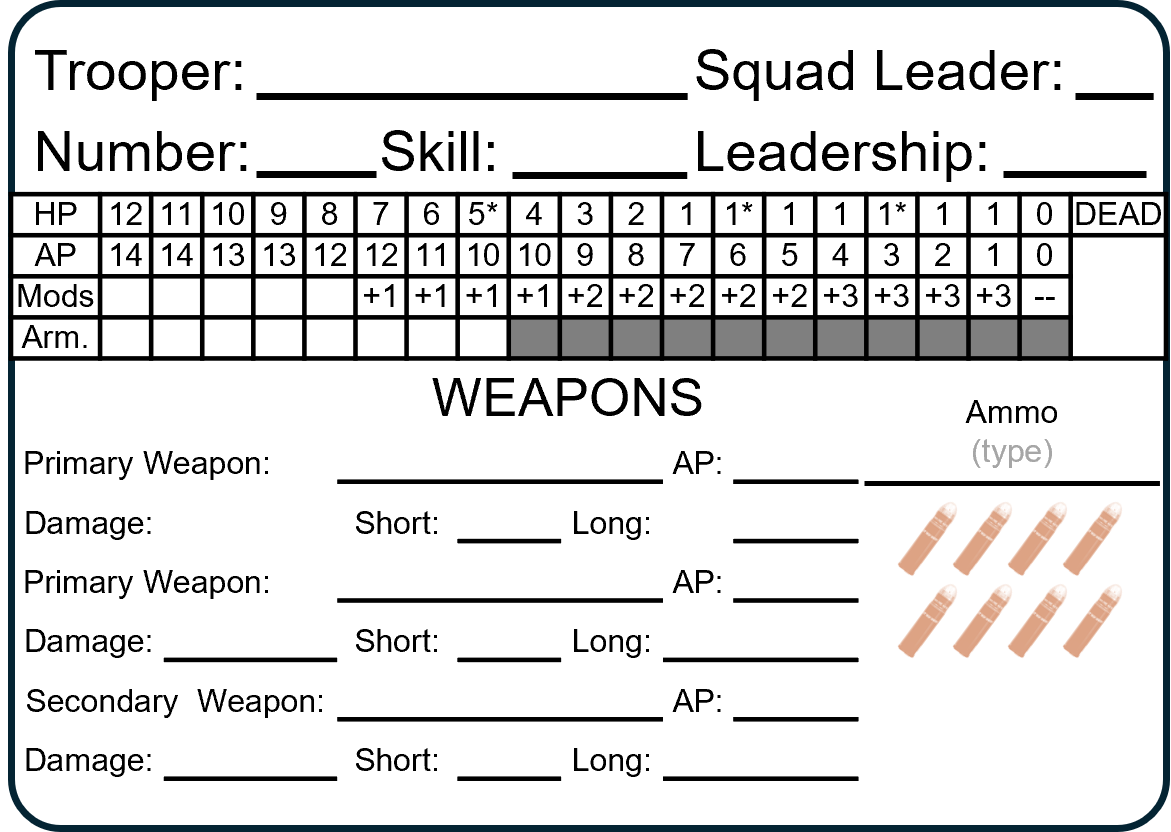
\includegraphics[alt='Sample Power Armor Trooper', width=5.63in, height=4in]{img/PowerArmorTrooper.png}
  \caption*{Power Armor Trooper Unit Card}
\end{figure}

There are a few key differences between the standard trooper unit card and a power armor trooper unit card.

Standard power armor has 6 cells of armor.
Basic power armor has only 4 cells of armor and heavy power armor has 8 cells of armor.
All other cells of armor should be marked off before the game.

Power armor troopers ignore bludgeoning damage (\textbackslash).
However, 9 or more points of bludgeoning damage in a single turn will knock a power armor trooper prone.
Standard damage (X) destroys armor before damaging HP cells.
If a single attack does more damage than the remaining armor, first mark all remaining armor and then mark HP cells starting with the 12 HP cell.

Once all of the armor has been destroyed, then the trooper's HP cells are marked.
Power armor protects the trooper, giving them more HP than a basic trooper.
HP cells are fully crossed out when the trooper takes standard damage (X).
The current HP of the trooper is given by the first cell to the right of the highest fully marked HP cell.
For example, if the trooper has HP 10, 9, and 6 marked off, their current HP is 5.
When marking damage, you still roll 2D6 and apply damage starting with the first unmarked HP cell to the right of the rolled value.

The HP cells marked with * indicate significant damage to the power armor.
When one of these cells is fully marked, the opponent may choose one of the weapon systems to disable on the power armor suit.
When two of these cells have been fully marked, the jet pack on the suit no longer functions.

Total action points (AP) for the trooper are given in the AP section.
Power armor greatly extends the capabilities of troopers, giving them more AP.
Use the value in the column corresponding to the trooper's current HP.
For example, if the trooper has 5 HP, then they have only 10 AP.

As with standard troopers, green troopers in power armor reduce all of their AP values by 1, while veteran troopers increase all values by 1 and elite troopers increase all values by 2.

Similarly, the modifier section tracks the current modifier for the trooper's target numbers based upon current HP.
For example, if the trooper has 5 HP, then add +1 to all target numbers.

Basic and standard power armor comes equipped with a jet pack.
Heavy power armor is too bulky to use a jet pack.

The weapons and equipment section list the primary and secondary weapons the trooper is equipped with, along with their damage values and range brackets.
Power armor troopers cannot use grenades but may use satchel changes.

The leadership section lists the squad leader for the trooper and their leadership score.
This section contains the information required for morale checks.


% --------------------------------------------------------------------------------
\subsubsection*{Weapons and Equipment}
% --------------------------------------------------------------------------------

Troopers carry one primary weapon, one secondary weapon, and 4 hand grenades.
All troopers have a helmet and combat knife.
The combat knife is assumed to be attached as a bayonet if the trooper is carrying a rifle or SMG.
Troopers may carry additional equipment in some cases.

\paragraph*{Primary Weapons}

Each trooper carries a single primary weapon.
Troopers can use the following primary weapons:

\begin{table}[H]
\ifthenelse{\not \equal{\outworldsMode}{mode-web}}{\fontfamily{Montserrat-LF}}{\small}\selectfont
\centering
\newcolumntype{R}[1]{>{\raggedleft\let\newline\\\arraybackslash\hspace{0pt}}m{#1}}
\begin{tabular}{!{\Vline{1pt}} m{6em} !{\Vline{1pt}} R{4.5em} !{\Vline{1pt}} R{6.5em} !{\Vline{1pt}} R{6.5em} !{\Vline{1pt}}}
\Hline{1pt}
\rowcolor{black!30}  \bfseries{Weapon} & \bfseries{Damage} & \bfseries{Short Range} & \bfseries{Long Range} \\
\Hline{1pt}
SMG*          & 3X &  5 &  17  \\
Rifle         & 4X & 26 &  85  \\
Laser SMG*    & 4X & 43 & 127  \\
Laser Rifle   & 5X & 66 & 232  \\
Long Rifle    & 6X & 30 & 102  \\
Gyrojet Rifle & 6X & 31 & 137  \\
\Hline{1pt}
\end{tabular}
\caption*{Primary Weapons}
\end{table}

Note, the SMG and Laser SMG are burst fire weapons and can fire into the same firing arc multiple times.
All other weapons may only fire into a firing arc once per turn.

\paragraph*{Secondary Weapons}

Each trooper may carry a single secondary weapon.
Troopers can use the following ranged secondary weapons:

\begin{table}[H]
\ifthenelse{\not \equal{\outworldsMode}{mode-web}}{\fontfamily{Montserrat-LF}}{\small}\selectfont
\centering
\newcolumntype{R}[1]{>{\raggedleft\let\newline\\\arraybackslash\hspace{0pt}}m{#1}}
\begin{tabular}{!{\Vline{1pt}} m{6em} !{\Vline{1pt}} R{4.5em} !{\Vline{1pt}} R{6.5em} !{\Vline{1pt}} R{6.5em} !{\Vline{1pt}}}
\Hline{1pt}
\rowcolor{black!30}  \bfseries{Weapon} & \bfseries{Damage} & \bfseries{Short Range} & \bfseries{Long Range} \\
\Hline{1pt}
Pistol        & 2X &  7 & 20  \\
Auto Pistol*  & 3X &  6 & 22  \\
Laser Pistol  & 4X & 11 & 40  \\
\Hline{1pt}
\end{tabular}
\caption*{Ranged Secondary Weapons}
\end{table}

Note, the auto pistol is a burst fire weapon and can fire into the same firing arc multiple times.
All other weapons may only fire into a firing arc once per turn.

Troopers can use the following melee secondary weapons:

\begin{table}[H]
\ifthenelse{\not \equal{\outworldsMode}{mode-web}}{\fontfamily{Montserrat-LF}}{\small}\selectfont
\centering
\newcolumntype{R}[1]{>{\raggedleft\let\newline\\\arraybackslash\hspace{0pt}}m{#1}}
\begin{tabular}{!{\Vline{1pt}} m{7.2em} !{\Vline{1pt}} R{5em} !{\Vline{1pt}} R{6.5em} !{\Vline{1pt}} R{6.5em} !{\Vline{1pt}}}
\Hline{1pt}
\rowcolor{black!30}  \bfseries{Weapon} & \bfseries{Damage} & \bfseries{Short Range} & \bfseries{Long Range} \\
\Hline{1pt}
Fists         & (AP/2)\textbackslash & 1 & --  \\
Bayonet/Knife & 3X                   & 1 & --  \\
Blackjack     & 5\textbackslash      & 1 & --  \\
Club          & 1X, 4\textbackslash  & 1 & --  \\
Stun Baton    & 8\textbackslash      & 1 & --  \\
Sword         & 4X                   & 1 & --  \\
Vibroblade    & 5X                   & 1 & --  \\
\Hline{1pt}
\end{tabular}
\caption*{Melee Secondary Weapons}
\end{table}

A trooper always has their fists and a bayonet/knife.
The other melee weapons take the place of a secondary weapon.

\paragraph*{Explosive Weapons}

Troopers can use the following explosives:

\begin{table}[H]
\ifthenelse{\not \equal{\outworldsMode}{mode-web}}{\fontfamily{Montserrat-LF}}{\small}\selectfont
\centering
\newcolumntype{R}[1]{>{\raggedleft\let\newline\\\arraybackslash\hspace{0pt}}m{#1}}
\begin{tabular}{!{\Vline{1pt}} m{8em} !{\Vline{1pt}} R{4.9em} !{\Vline{1pt}} R{4.1em} !{\Vline{1pt}} R{4em} !{\Vline{1pt}} R{6.5em} !{\Vline{1pt}} R{6.5em} !{\Vline{1pt}}}
\Hline{1pt}
\rowcolor{black!30}  \bfseries{Weapon} & \bfseries{Damage} & \bfseries{AP Cost} & \bfseries{Ammo} & \bfseries{Short Range} & \bfseries{Long Range} \\
\Hline{1pt}
Hand Grenade   &    6X/3X/1X & AP      & 4 & AP   & --  \\
Satchel Charge &   10X/5X/2X & 3 or AP & 1 & AP/2 & --  \\
\Hline{1pt}
\end{tabular}
\caption*{Explosive Weapons}
\end{table}

The ammo column indicates how many rounds of ammunition come with the weapon.
The damage is given is descending order for the point of detonation, the adjacent dots, the dots 2 away from the detonation, and so on.
It takes 1 AP per dot to throw a hand grenade and it takes 2 AP per dot to throw a satchel charge.

A trooper carries 4 grenades in addition to their primary and secondary weapons.
A satchel charge is a secondary weapon, so a trooper cannot carry a ranged or melee secondary weapon if they are carrying a satchel charge.

\paragraph*{Body Armor}

Troopers can wear body armor.
A trooper ignores bludgeoning damage while wearing body armor and any cells of armor are destroyed before applying lethal damage to the trooper.

\begin{table}[H]
\ifthenelse{\not \equal{\outworldsMode}{mode-web}}{\fontfamily{Montserrat-LF}}{\small}\selectfont
\centering
\newcolumntype{R}[1]{>{\raggedleft\let\newline\\\arraybackslash\hspace{0pt}}m{#1}}
\begin{tabular}{!{\Vline{1pt}} m{6.5em} !{\Vline{1pt}} R{5em} !{\Vline{1pt}} R{4.5em} !{\Vline{1pt}}}
\Hline{1pt}
\rowcolor{black!30}  \bfseries{Armor Type} & \bfseries{Coverage} & \bfseries{AP Cost} \\
\Hline{1pt}
Basic    & 2 & 1  \\
Standard & 4 & 2  \\
Heavy    & 6 & 3  \\
\Hline{1pt}
\end{tabular}
\caption*{Body Armor AP Costs}
\end{table}

To equip body armor on a trooper, indicate the number of cells of body armor on the unit card and mark off all other cells of armor before the game.
Reduce the trooper's AP to account for the body armor.
For example, with standard body armor, leave 4 cells of armor on the unit card and reduce all values in the AP row by 2.


% --------------------------------------------------------------------------------
\subsubsection*{Movement}
% --------------------------------------------------------------------------------

Troopers may move and take special actions prior to taking any combat actions.

\paragraph*{Basic Movement}

Troopers can use a maximum of 8 AP for movement.
Troopers move between adjacent dots on the map so long as the the new location is on valid terrain and the path between the dots does not pass though an impassible obstacle, such as a solid high wall or the truck of a tree.

Movement between adjacent dots with no obstructions between them costs 1 AP.
Movement between adjacent dots with an obstruction between costs 2 AP.
Obstructions include objects that are shorter than a person, such as furniture, light vegetation, and low walls.

Troopers may only enter and exit buildings through doorways and windows.
Movement between adjacent dots that passes through a doorway costs 2 AP.
Movement between adjacent dots that passes through a window costs 4 AP; however troopers cannot voluntarily fall out of an upper story window or off of a building.

Troopers may use stairs and ladders to change levels in or on a building.
Movement between levels costs 3 AP.
The trooper stays on the same dot when changing levels.
The current level of the trooper should be tracked on the unit card or next to the miniature.

Troopers may hide behind solid obstructions, such as furniture and low walls.
It costs 1 AP to go prone.
It costs 2 AP to stand from a prone position.
Movement while prone costs double the standard AP.

\begin{table}[H]
\ifthenelse{\not \equal{\outworldsMode}{mode-web}}{\fontfamily{Montserrat-LF}}{\small}\selectfont
\centering
\newcolumntype{R}[1]{>{\raggedleft\let\newline\\\arraybackslash\hspace{0pt}}m{#1}}
\begin{tabular}{!{\Vline{1pt}} m{9em} !{\Vline{1pt}} R{4.5em} !{\Vline{1pt}}}
\Hline{1pt}
\rowcolor{black!30}  \bfseries{Movement Type} & \bfseries{AP Cost} \\
\Hline{1pt}
Standard         & 1   \\
Obstructed       & 2   \\
Through door     & 2   \\
Through window   & 4   \\
Change level     & 3   \\
Go prone         & 1   \\
Stand from prone & 2   \\
Move while prone & 2x  \\
\Hline{1pt}
\end{tabular}
\caption*{Movement AP Costs}
\end{table}

\paragraph*{Special Actions}

A trooper may take the following special actions during their movement:

\begin{table}[H]
\ifthenelse{\not \equal{\outworldsMode}{mode-web}}{\fontfamily{Montserrat-LF}}{\small}\selectfont
\centering
\newcolumntype{R}[1]{>{\raggedleft\let\newline\\\arraybackslash\hspace{0pt}}m{#1}}
\begin{tabular}{!{\Vline{1pt}} m{11em} !{\Vline{1pt}} R{4.5em} !{\Vline{1pt}}}
\Hline{1pt}
\rowcolor{black!30}  \bfseries{Action} & \bfseries{AP Cost} \\
\Hline{1pt}
Change Weapon      & 3  \\
Exchange Equipment & 6  \\
\Hline{1pt}
\end{tabular}
\caption*{Special Action AP Costs}
\end{table}

A trooper can only have one weapon active at a time.
It costs 3 AP to change active weapons, including to change to an explosive.
A trooper automatically switches back to their primary or secondary weapon after using a grenade or satchel charge, for 0 AP.

Troopers may exchange weapons or equipment.
It costs 6 AP to take a weapon or equipment from another trooper, including a dead or unconscious trooper.
A trooper cannot exceed the basic carrying capabilities given on their unit card.
A trooper may drop weapons or equipment for 0 AP; however, any trooper, friendly or enemy, may pick up the dropped weapon or equipment.


% --------------------------------------------------------------------------------
\subsubsection*{Combat}
% --------------------------------------------------------------------------------

Power armor troopers largely use the same rules as standard troopers.

\paragraph*{Firing Arcs}

Power armor troopers may place firing arcs for all of their weapons.
If a weapon does not have a firing arc, then that weapon cannot fire.
If one of a power armor trooper's weapons is an explosive, this trooper may use the explosive and establish firing arcs with their other weapons.

\paragraph*{Hand to Hand Combat}

It costs 5 AP to make a hand to hand attack.
Power armor trooper fists are more effective at dealing damage.

\begin{table}[H]
\ifthenelse{\not \equal{\outworldsMode}{mode-web}}{\fontfamily{Montserrat-LF}}{\small}\selectfont
\centering
\newcolumntype{R}[1]{>{\raggedleft\let\newline\\\arraybackslash\hspace{0pt}}m{#1}}
\begin{tabular}{!{\Vline{1pt}} m{6em} !{\Vline{1pt}} R{5em} !{\Vline{1pt}} R{6.5em} !{\Vline{1pt}} R{6.5em} !{\Vline{1pt}}}
\Hline{1pt}
\rowcolor{black!30}  \bfseries{Weapon} & \bfseries{Damage} & \bfseries{Short Range} & \bfseries{Long Range} \\
\Hline{1pt}
Fists         & 1X, (AP/2)\textbackslash & 1 & - \\
\Hline{1pt}
\end{tabular}
\caption*{Power Armor Hand to Hand}
\end{table}

\paragraph*{Explosives}

Power armor troopers may use explosive weapons, but may not use hand grenades or smoke grenades.
Power armor troopers may pick up and use satchel charges.



\newpage

% --------------------------------------------------------------------------------
\newsection{Advanced Infantry}{advanced-infantry}
% --------------------------------------------------------------------------------

Infantry troopers can wear power armor in \emph{Skirmishers}.
This section relies upon rules from the Advanced Infantry section.


% --------------------------------------------------------------------------------
\subsubsection*{Unit Card}
% --------------------------------------------------------------------------------

The unit card shows the current capabilities of a trooper in power armor and tracks damage.
A unit card can be formatted in any way so long as it contains all the essential information.
Below is a sample unit card for a power armor trooper.

\begin{figure}[H]
  \centering
  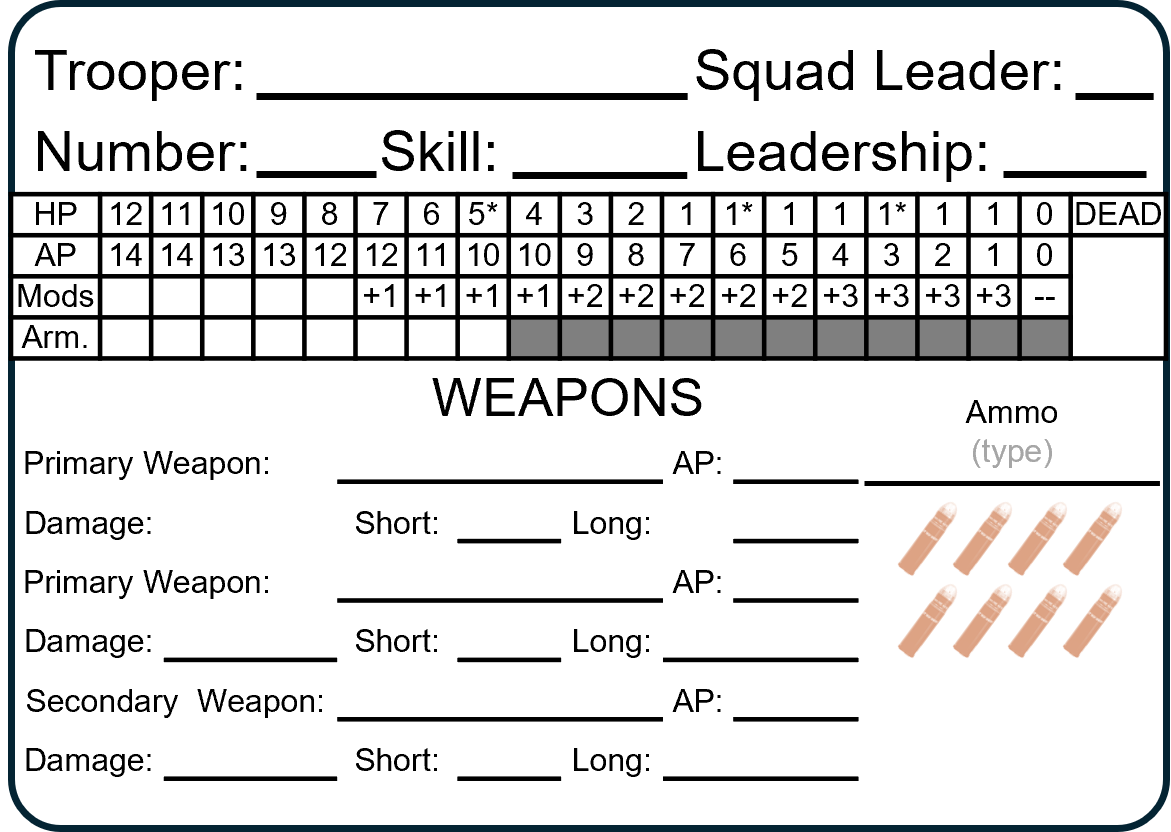
\includegraphics[alt='Sample Power Armor Trooper', width=5.63in, height=4in]{img/PowerArmorTrooper.png}
  \caption*{Power Armor Trooper Unit Card}
\end{figure}

There are a few key differences between the standard trooper unit card and a power armor trooper unit card.

Standard power armor has 6 cells of armor.
Basic power armor has only 4 cells of armor and heavy power armor has 8 cells of armor.
All other cells of armor should be marked off before the game.

Power armor troopers ignore bludgeoning damage (\textbackslash).
However, 9 or more points of bludgeoning damage in a single turn will knock a power armor trooper prone.
Standard damage (X) destroys armor before damaging HP cells.
If a single attack does more damage than the remaining armor, first mark all remaining armor and then mark HP cells starting with the 12 HP cell.

Once all of the armor has been destroyed, then the trooper's HP cells are marked.
Power armor protects the trooper, giving them more HP than a basic trooper.
HP cells are fully crossed out when the trooper takes standard damage (X).
The current HP of the trooper is given by the first cell to the right of the highest fully marked HP cell.
For example, if the trooper has HP 10, 9, and 6 marked off, their current HP is 5.
When marking damage, you still roll 2D6 and apply damage starting with the first unmarked HP cell to the right of the rolled value.

The HP cells marked with * indicate significant damage to the power armor.
When one of these cells is fully marked, the opponent may choose one of the weapon systems to disable on the power armor suit.
When two of these cells have been fully marked, the jet pack on the suit no longer functions.

Total action points (AP) for the trooper are given in the AP section.
Power armor greatly extends the capabilities of troopers, giving them more AP.
Use the value in the column corresponding to the trooper's current HP.
For example, if the trooper has 5 HP, then they have only 10 AP.

As with standard troopers, green troopers in power armor reduce all of their AP values by 1, while veteran troopers increase all values by 1 and elite troopers increase all values by 2.

Similarly, the modifier section tracks the current modifier for the trooper's target numbers based upon current HP.
For example, if the trooper has 5 HP, then add +1 to all target numbers.

Basic and standard power armor comes equipped with a jet pack.
Heavy power armor is too bulky to use a jet pack.

The weapons and equipment section list the primary and secondary weapons the trooper is equipped with, along with their damage values and range brackets.
Power armor troopers cannot use grenades but may use satchel changes.

The leadership section lists the squad leader for the trooper and their leadership score.
This section contains the information required for morale checks.


% --------------------------------------------------------------------------------
\subsubsection*{Weapons and Equipment}
% --------------------------------------------------------------------------------

Troopers carry one primary weapon, one secondary weapon, and 4 hand grenades.
All troopers have a helmet and combat knife.
The combat knife is assumed to be attached as a bayonet if the trooper is carrying a rifle or SMG.
Troopers may carry additional equipment in some cases.

\paragraph*{Primary Weapons}

Each trooper carries a single primary weapon.
Troopers can use the following primary weapons:

\begin{table}[H]
\ifthenelse{\not \equal{\outworldsMode}{mode-web}}{\fontfamily{Montserrat-LF}}{\small}\selectfont
\centering
\newcolumntype{R}[1]{>{\raggedleft\let\newline\\\arraybackslash\hspace{0pt}}m{#1}}
\begin{tabular}{!{\Vline{1pt}} m{6em} !{\Vline{1pt}} R{4.5em} !{\Vline{1pt}} R{6.5em} !{\Vline{1pt}} R{6.5em} !{\Vline{1pt}}}
\Hline{1pt}
\rowcolor{black!30}  \bfseries{Weapon} & \bfseries{Damage} & \bfseries{Short Range} & \bfseries{Long Range} \\
\Hline{1pt}
SMG*          & 3X &  5 &  17  \\
Rifle         & 4X & 26 &  85  \\
Laser SMG*    & 4X & 43 & 127  \\
Laser Rifle   & 5X & 66 & 232  \\
Long Rifle    & 6X & 30 & 102  \\
Gyrojet Rifle & 6X & 31 & 137  \\
\Hline{1pt}
\end{tabular}
\caption*{Primary Weapons}
\end{table}

Note, the SMG and Laser SMG are burst fire weapons and can fire into the same firing arc multiple times.
All other weapons may only fire into a firing arc once per turn.

\paragraph*{Secondary Weapons}

Each trooper may carry a single secondary weapon.
Troopers can use the following ranged secondary weapons:

\begin{table}[H]
\ifthenelse{\not \equal{\outworldsMode}{mode-web}}{\fontfamily{Montserrat-LF}}{\small}\selectfont
\centering
\newcolumntype{R}[1]{>{\raggedleft\let\newline\\\arraybackslash\hspace{0pt}}m{#1}}
\begin{tabular}{!{\Vline{1pt}} m{6em} !{\Vline{1pt}} R{4.5em} !{\Vline{1pt}} R{6.5em} !{\Vline{1pt}} R{6.5em} !{\Vline{1pt}}}
\Hline{1pt}
\rowcolor{black!30}  \bfseries{Weapon} & \bfseries{Damage} & \bfseries{Short Range} & \bfseries{Long Range} \\
\Hline{1pt}
Pistol        & 2X &  7 & 20  \\
Auto Pistol*  & 3X &  6 & 22  \\
Laser Pistol  & 4X & 11 & 40  \\
\Hline{1pt}
\end{tabular}
\caption*{Ranged Secondary Weapons}
\end{table}

Note, the auto pistol is a burst fire weapon and can fire into the same firing arc multiple times.
All other weapons may only fire into a firing arc once per turn.

Troopers can use the following melee secondary weapons:

\begin{table}[H]
\ifthenelse{\not \equal{\outworldsMode}{mode-web}}{\fontfamily{Montserrat-LF}}{\small}\selectfont
\centering
\newcolumntype{R}[1]{>{\raggedleft\let\newline\\\arraybackslash\hspace{0pt}}m{#1}}
\begin{tabular}{!{\Vline{1pt}} m{7.2em} !{\Vline{1pt}} R{5em} !{\Vline{1pt}} R{6.5em} !{\Vline{1pt}} R{6.5em} !{\Vline{1pt}}}
\Hline{1pt}
\rowcolor{black!30}  \bfseries{Weapon} & \bfseries{Damage} & \bfseries{Short Range} & \bfseries{Long Range} \\
\Hline{1pt}
Fists         & (AP/2)\textbackslash & 1 & --  \\
Bayonet/Knife & 3X                   & 1 & --  \\
Blackjack     & 5\textbackslash      & 1 & --  \\
Club          & 1X, 4\textbackslash  & 1 & --  \\
Stun Baton    & 8\textbackslash      & 1 & --  \\
Sword         & 4X                   & 1 & --  \\
Vibroblade    & 5X                   & 1 & --  \\
\Hline{1pt}
\end{tabular}
\caption*{Melee Secondary Weapons}
\end{table}

A trooper always has their fists and a bayonet/knife.
The other melee weapons take the place of a secondary weapon.

\paragraph*{Explosive Weapons}

Troopers can use the following explosives:

\begin{table}[H]
\ifthenelse{\not \equal{\outworldsMode}{mode-web}}{\fontfamily{Montserrat-LF}}{\small}\selectfont
\centering
\newcolumntype{R}[1]{>{\raggedleft\let\newline\\\arraybackslash\hspace{0pt}}m{#1}}
\begin{tabular}{!{\Vline{1pt}} m{8em} !{\Vline{1pt}} R{4.9em} !{\Vline{1pt}} R{4.1em} !{\Vline{1pt}} R{4em} !{\Vline{1pt}} R{6.5em} !{\Vline{1pt}} R{6.5em} !{\Vline{1pt}}}
\Hline{1pt}
\rowcolor{black!30}  \bfseries{Weapon} & \bfseries{Damage} & \bfseries{AP Cost} & \bfseries{Ammo} & \bfseries{Short Range} & \bfseries{Long Range} \\
\Hline{1pt}
Hand Grenade   &    6X/3X/1X & AP      & 4 & AP   & --  \\
Satchel Charge &   10X/5X/2X & 3 or AP & 1 & AP/2 & --  \\
\Hline{1pt}
\end{tabular}
\caption*{Explosive Weapons}
\end{table}

The ammo column indicates how many rounds of ammunition come with the weapon.
The damage is given is descending order for the point of detonation, the adjacent dots, the dots 2 away from the detonation, and so on.
It takes 1 AP per dot to throw a hand grenade and it takes 2 AP per dot to throw a satchel charge.

A trooper carries 4 grenades in addition to their primary and secondary weapons.
A satchel charge is a secondary weapon, so a trooper cannot carry a ranged or melee secondary weapon if they are carrying a satchel charge.

\paragraph*{Body Armor}

Troopers can wear body armor.
A trooper ignores bludgeoning damage while wearing body armor and any cells of armor are destroyed before applying lethal damage to the trooper.

\begin{table}[H]
\ifthenelse{\not \equal{\outworldsMode}{mode-web}}{\fontfamily{Montserrat-LF}}{\small}\selectfont
\centering
\newcolumntype{R}[1]{>{\raggedleft\let\newline\\\arraybackslash\hspace{0pt}}m{#1}}
\begin{tabular}{!{\Vline{1pt}} m{6.5em} !{\Vline{1pt}} R{5em} !{\Vline{1pt}} R{4.5em} !{\Vline{1pt}}}
\Hline{1pt}
\rowcolor{black!30}  \bfseries{Armor Type} & \bfseries{Coverage} & \bfseries{AP Cost} \\
\Hline{1pt}
Basic    & 2 & 1  \\
Standard & 4 & 2  \\
Heavy    & 6 & 3  \\
\Hline{1pt}
\end{tabular}
\caption*{Body Armor AP Costs}
\end{table}

To equip body armor on a trooper, indicate the number of cells of body armor on the unit card and mark off all other cells of armor before the game.
Reduce the trooper's AP to account for the body armor.
For example, with standard body armor, leave 4 cells of armor on the unit card and reduce all values in the AP row by 2.


% --------------------------------------------------------------------------------
\subsubsection*{Movement}
% --------------------------------------------------------------------------------

Troopers may move and take special actions prior to taking any combat actions.

\paragraph*{Basic Movement}

Troopers can use a maximum of 8 AP for movement.
Troopers move between adjacent dots on the map so long as the the new location is on valid terrain and the path between the dots does not pass though an impassible obstacle, such as a solid high wall or the truck of a tree.

Movement between adjacent dots with no obstructions between them costs 1 AP.
Movement between adjacent dots with an obstruction between costs 2 AP.
Obstructions include objects that are shorter than a person, such as furniture, light vegetation, and low walls.

Troopers may only enter and exit buildings through doorways and windows.
Movement between adjacent dots that passes through a doorway costs 2 AP.
Movement between adjacent dots that passes through a window costs 4 AP; however troopers cannot voluntarily fall out of an upper story window or off of a building.

Troopers may use stairs and ladders to change levels in or on a building.
Movement between levels costs 3 AP.
The trooper stays on the same dot when changing levels.
The current level of the trooper should be tracked on the unit card or next to the miniature.

Troopers may hide behind solid obstructions, such as furniture and low walls.
It costs 1 AP to go prone.
It costs 2 AP to stand from a prone position.
Movement while prone costs double the standard AP.

\begin{table}[H]
\ifthenelse{\not \equal{\outworldsMode}{mode-web}}{\fontfamily{Montserrat-LF}}{\small}\selectfont
\centering
\newcolumntype{R}[1]{>{\raggedleft\let\newline\\\arraybackslash\hspace{0pt}}m{#1}}
\begin{tabular}{!{\Vline{1pt}} m{9em} !{\Vline{1pt}} R{4.5em} !{\Vline{1pt}}}
\Hline{1pt}
\rowcolor{black!30}  \bfseries{Movement Type} & \bfseries{AP Cost} \\
\Hline{1pt}
Standard         & 1   \\
Obstructed       & 2   \\
Through door     & 2   \\
Through window   & 4   \\
Change level     & 3   \\
Go prone         & 1   \\
Stand from prone & 2   \\
Move while prone & 2x  \\
\Hline{1pt}
\end{tabular}
\caption*{Movement AP Costs}
\end{table}

\paragraph*{Special Actions}

A trooper may take the following special actions during their movement:

\begin{table}[H]
\ifthenelse{\not \equal{\outworldsMode}{mode-web}}{\fontfamily{Montserrat-LF}}{\small}\selectfont
\centering
\newcolumntype{R}[1]{>{\raggedleft\let\newline\\\arraybackslash\hspace{0pt}}m{#1}}
\begin{tabular}{!{\Vline{1pt}} m{11em} !{\Vline{1pt}} R{4.5em} !{\Vline{1pt}}}
\Hline{1pt}
\rowcolor{black!30}  \bfseries{Action} & \bfseries{AP Cost} \\
\Hline{1pt}
Change Weapon      & 3  \\
Exchange Equipment & 6  \\
\Hline{1pt}
\end{tabular}
\caption*{Special Action AP Costs}
\end{table}

A trooper can only have one weapon active at a time.
It costs 3 AP to change active weapons, including to change to an explosive.
A trooper automatically switches back to their primary or secondary weapon after using a grenade or satchel charge, for 0 AP.

Troopers may exchange weapons or equipment.
It costs 6 AP to take a weapon or equipment from another trooper, including a dead or unconscious trooper.
A trooper cannot exceed the basic carrying capabilities given on their unit card.
A trooper may drop weapons or equipment for 0 AP; however, any trooper, friendly or enemy, may pick up the dropped weapon or equipment.


% --------------------------------------------------------------------------------
\subsubsection*{Combat}
% --------------------------------------------------------------------------------

Power armor troopers largely use the same rules as standard troopers.

\paragraph*{Firing Arcs}

Power armor troopers may place firing arcs for all of their weapons.
If a weapon does not have a firing arc, then that weapon cannot fire.
If one of a power armor trooper's weapons is an explosive, this trooper may use the explosive and establish firing arcs with their other weapons.

\paragraph*{Hand to Hand Combat}

It costs 5 AP to make a hand to hand attack.
Power armor trooper fists are more effective at dealing damage.

\begin{table}[H]
\ifthenelse{\not \equal{\outworldsMode}{mode-web}}{\fontfamily{Montserrat-LF}}{\small}\selectfont
\centering
\newcolumntype{R}[1]{>{\raggedleft\let\newline\\\arraybackslash\hspace{0pt}}m{#1}}
\begin{tabular}{!{\Vline{1pt}} m{6em} !{\Vline{1pt}} R{5em} !{\Vline{1pt}} R{6.5em} !{\Vline{1pt}} R{6.5em} !{\Vline{1pt}}}
\Hline{1pt}
\rowcolor{black!30}  \bfseries{Weapon} & \bfseries{Damage} & \bfseries{Short Range} & \bfseries{Long Range} \\
\Hline{1pt}
Fists         & 1X, (AP/2)\textbackslash & 1 & - \\
\Hline{1pt}
\end{tabular}
\caption*{Power Armor Hand to Hand}
\end{table}

\paragraph*{Explosives}

Power armor troopers may use explosive weapons, but may not use hand grenades or smoke grenades.
Power armor troopers may pick up and use satchel charges.



\newpage

% --------------------------------------------------------------------------------
\newsection{Sample Unit Cards}{sample-unit-cards}
% --------------------------------------------------------------------------------

\begin{figure}[!h]
  \centering
  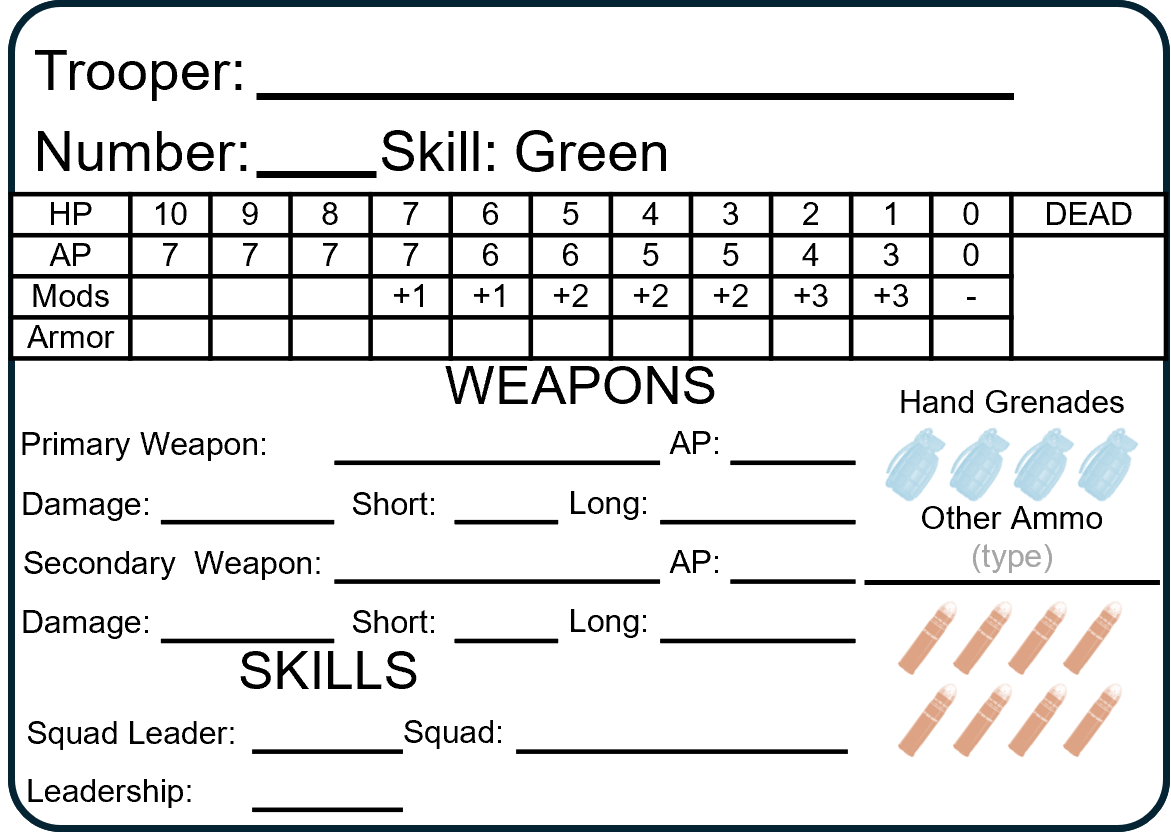
\includegraphics[alt='Sample Green Trooper', width=5.63in, height=4in]{img/GreenTrooper.png}
  \caption*{Sample Green Trooper}
\end{figure}

\begin{figure}[!h]
  \centering
  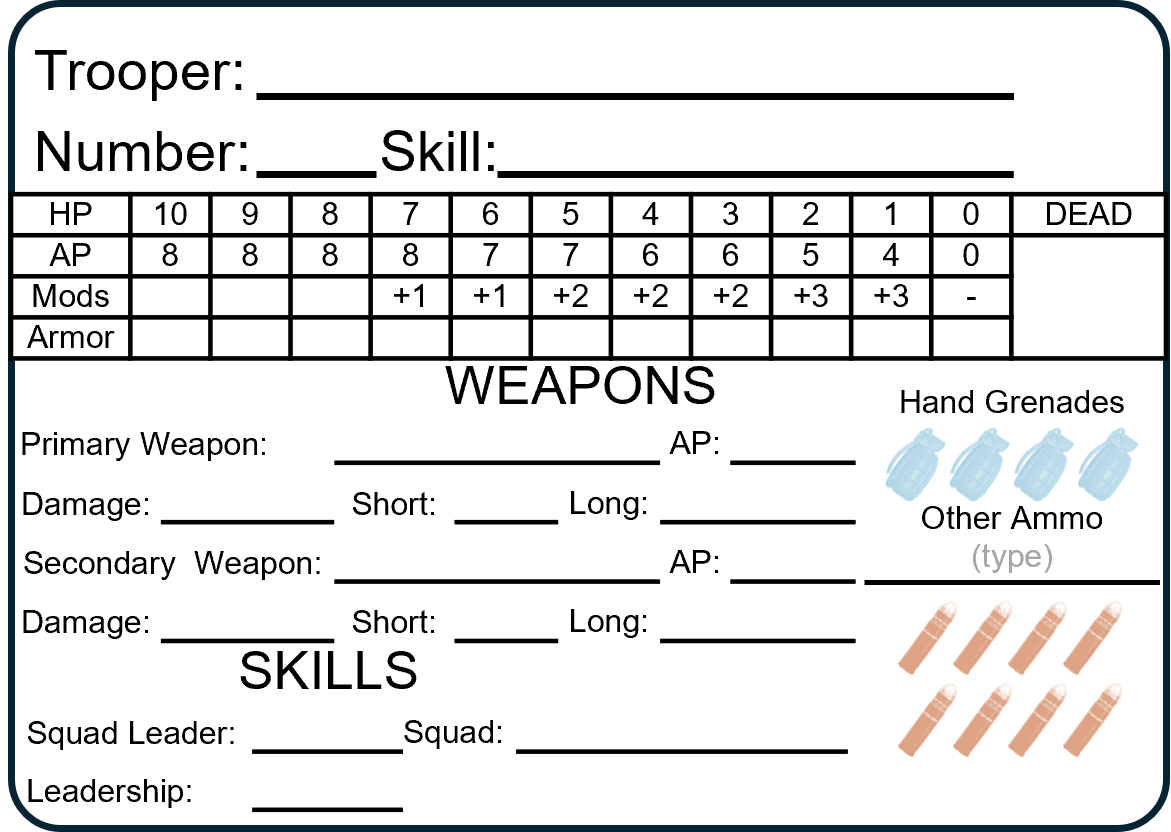
\includegraphics[alt='Sample Regular Trooper', width=5.63in, height=4in]{img/RegularTrooper.png}
  \caption*{Sample Regular Trooper}
\end{figure}

\begin{figure}[!h]
  \centering
  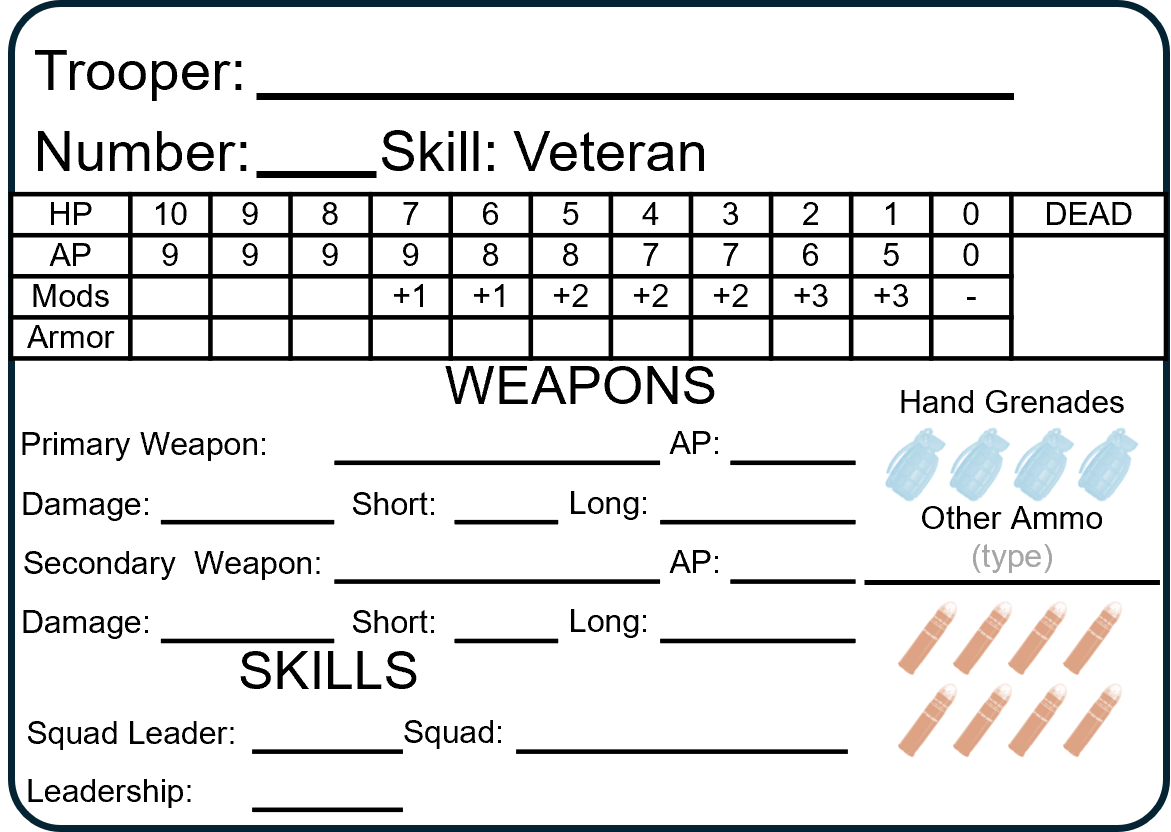
\includegraphics[alt='Sample Veteran Trooper', width=5.63in, height=4in]{img/VeteranTrooper.png}
  \caption*{Sample Veteran Trooper}
\end{figure}

\begin{figure}[!h]
  \centering
  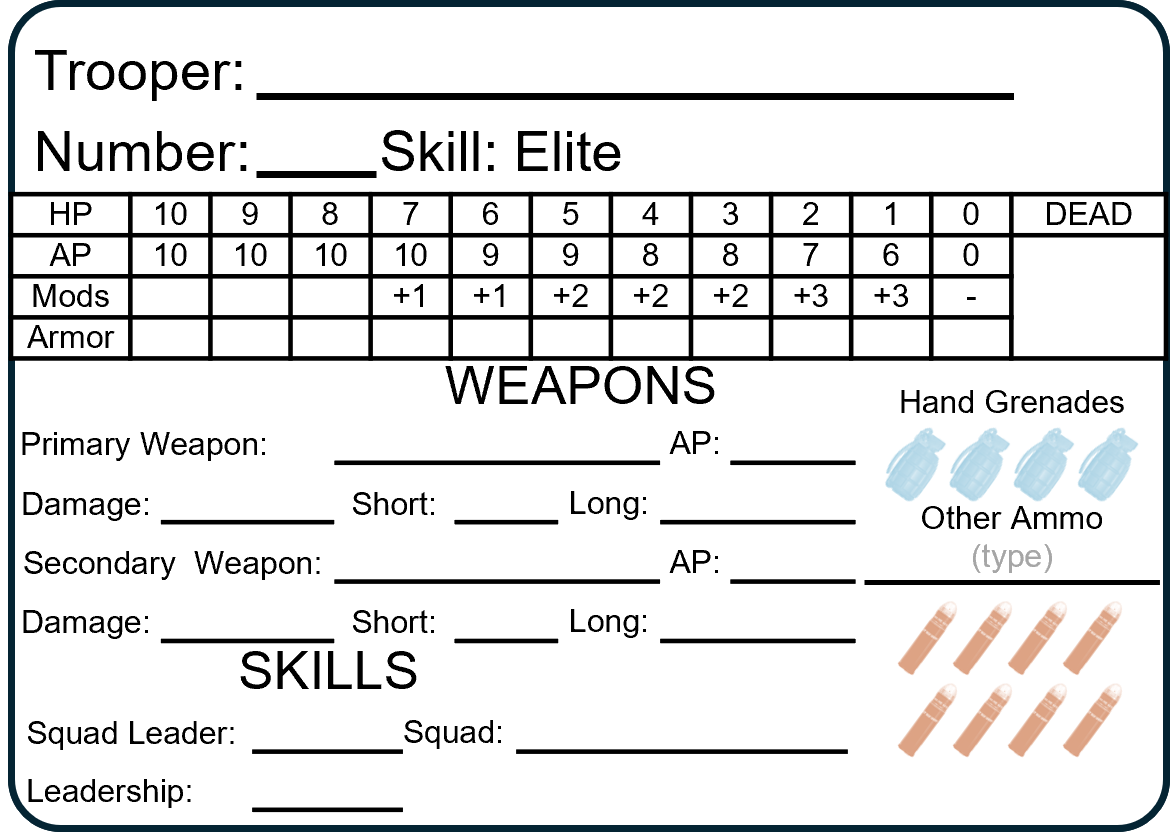
\includegraphics[alt='Sample Elite Trooper', width=5.63in, height=4in]{img/EliteTrooper.png}
  \caption*{Sample Elite Trooper}
\end{figure}


\newpage

% --------------------------------------------------------------------------------
\newsection{Downloads}{downloads}
\label{sec:downloads}
% --------------------------------------------------------------------------------

% --------------------------------------------------------------------------------
% Core downloads
% --------------------------------------------------------------------------------

These rules may be downloaded in PDF format:

\ifthenelse{\equal{\outworldsMode}{mode-web}}{
\HCode{
<iframe
  class="itchio-frame"
  frameborder="0"
  src="https://itch.io/embed/2771729?bg_color=ccc5b3&amp;fg_color=000000&amp;link_color=313831&amp;border_color=363636"
  width="552"
  height="167"
>
<a
  href="https://jeremyluket.itch.io/skirmishers"
>
Skirmishers by JeremyLT
</a>
</iframe>
}}{}

\begin{itemize}

\item \emph{Full}: \href{https://raw.githubusercontent.com/Eudicods/skirmishers/rules-pdf/skirmishers.pdf}{Full rules}

\end{itemize}

% --------------------------------------------------------------------------------
% GitHub
% --------------------------------------------------------------------------------

The source files for \emph{Skirmishers} are on \href{https://github.com/Eudicods/skirmishers}{GitHub}.


\newpage
\end{document}
% --------------------------------------------------------------------------------
